
\documentclass[letterpaper, reqno,11pt]{article}
\usepackage[margin=1.0in]{geometry}
\usepackage{color,latexsym,amsmath,amssymb}
\usepackage{fancyhdr}
\usepackage{amsthm}
\usepackage[linesnumbered,lined,boxed,commentsnumbered,noend,noline]{algorithm2e}
\usepackage{dsfont}
\usepackage{graphicx}
\usepackage{hyperref}
\usepackage{bbm}
\usepackage[inline]{enumitem}
\usepackage[numbers]{natbib}
\usepackage{framed}
\usepackage{titling}
\usepackage{subcaption}
\usepackage[dvipsnames]{xcolor}
\usepackage{tikz}
\usetikzlibrary{hobby}
\usetikzlibrary{shapes.multipart}
\usepackage{pgfplots}
\pgfplotsset{compat=1.7}
\usetikzlibrary{arrows.meta}
\usetikzlibrary{decorations.markings}
\usetikzlibrary{shapes}
\usetikzlibrary{arrows}
\usepgfplotslibrary{fillbetween}
\usetikzlibrary{patterns}

\tikzset{invclip/.style={clip,insert path={{[reset cm]
  (-16383.99999pt,-16383.99999pt) rectangle (16383.99999pt,16383.99999pt)}}}}

\allowdisplaybreaks

\newcommand{\RR}{\mathbb{R}}
\newcommand{\CC}{\mathbb{C}}
\newcommand{\ZZ}{\mathbb{Z}}
\newcommand{\QQ}{\mathbb{Q}}
\newcommand{\NN}{\mathbb{N}}
\newcommand{\FF}{\mathbb{F}}
\newcommand{\PP}{\mathop{{}\mathbb{P}}}
\newcommand{\EE}{\mathop{{}\mathbb{E}}}
\newcommand{\LL}{\mathbb{L}}
\newcommand{\TT}{\mathbb{T}}
\newcommand{\GI}{\textrm{GI}}
\newcommand{\coGI}{\overline{\textrm{GI}}}
\DeclareMathOperator{\conv}{conv}
\DeclareMathOperator{\charcone}{char.cone}
\DeclareMathOperator{\STAB}{STAB}
\DeclareMathOperator{\Down}{Down}
\DeclareMathOperator{\lca}{lca}
\DeclareMathOperator{\ex}{ex}
\DeclareMathOperator{\Span}{span}
\DeclareMathOperator{\T}{T}
\DeclareMathOperator{\F}{F}
\DeclareMathOperator{\shP}{\# P}
\DeclareMathOperator{\shSAT}{\# SAT}
\DeclareMathOperator{\shDNF}{\# DNF}
\DeclareMathOperator{\DNF}{DNF}
\DeclareMathOperator{\Poly}{P}
\DeclareMathOperator{\CNF}{CNF}
\DeclareMathOperator{\SAT}{SAT}
\DeclareMathOperator{\BPP}{BPP}
\DeclareMathOperator{\poly}{poly}
\DeclareMathOperator{\RP}{RP}
\DeclareMathOperator{\EXP}{EXP}
\DeclareMathOperator{\DTIME}{DTIME}
\DeclareMathOperator{\NP}{NP}
\DeclareMathOperator{\MCprime}{MC'}
\DeclareMathOperator{\Var}{Var}
\DeclareMathOperator{\IP}{IP}
\DeclareMathOperator{\PSPACE}{PSPACE}
\DeclareMathOperator{\lollipop}{lollipop}
\DeclareMathOperator{\ustconn}{\textsc{UST-Conn}}
\DeclareMathOperator{\RL}{RL}
\newcommand\mycommfont[1]{\ttfamily\textcolor{blue}{#1}}
\SetCommentSty{mycommfont}
\SetKwFor{RepTimes}{repeat}{times}{end}
\begin{document}
\pagenumbering{arabic}
\title{Lectures on Linearity Testing}
\author{Yuchong Pan}
\date{\today}
\newtheorem{theorem}{Theorem}
\newtheorem{lemma}[theorem]{Lemma}
\newtheorem{proposition}[theorem]{Proposition}
\newtheorem{corollary}[theorem]{Corollary}
\newtheorem{fact}[theorem]{Fact}
\newtheorem{problem}[theorem]{Problem}
\newtheorem{observation}[theorem]{Observation}
\newtheorem{claim}{Claim}
\newtheorem{exercise}{Exercise}
\theoremstyle{definition}
\newtheorem{definition}[theorem]{Definition}
%\maketitle
%

\begin{framed}
\noindent{\bf 6.842 Randomness and Computation} \hfill \thedate
\begin{center}
\Large{\thetitle}
\end{center}
\noindent{\em Lecturer: Ronitt Rubinfield} \hfill {\em Scribe: \theauthor}
\end{framed}

\section{Linearity Testing}

\begin{definition}
  Let $G$ and $H$ be finite groups. Let $f : G \to H$. Then $f$ is said to be \emph{linear} (i.e., is a \emph{homomorphism}) if for all $x, y \in G$,
  $$ f(x) +_H f(y) =_H f\left(x +_G y\right). $$
  For all $\varepsilon > 0$, $f$ is said to be \emph{$\varepsilon$-linear} if there exists a linear function $g : G \to H$ such that $f$ and $g$ agree on at least $1 - \varepsilon$ fraction of inputs in $G$, i.e.,
  $$ \PP_{x \in G}[f(x) = g(x)] \geq 1 - \varepsilon, $$
  or equivalently,
  $$ \frac{|\{ x \in G : f(x) = g(x) \}|}{|G|} \geq 1 - \varepsilon. $$
\end{definition}

Algorithm \ref{alg:proposed-lintest} is a natural test for the linearity of a function $f : G \to H$, where $G$ and $H$ are finite groups.

\begin{algorithm}
  \RepTimes{?}{
    pick random $x, y \in G$ \\
    \If{$f(x) + f(y) \neq f(x + y)$}
    {
      \Return{``fail''}
    }
  }
  \Return{``pass''}
  \caption{A proposed test for the linearity of a function $f : G \to H$, where $G$ and $H$ are finite groups.}
  \label{alg:proposed-lintest}
\end{algorithm}

\begin{observation} \label{obs:uniform}
  Let $G$ be a finite group. For all $a, y \in G$, $\PP_{x \in G}[y = a + x] = 1/|G|$. In other words, if $x$ is chosen uniformly from $G$, then $a + x$ is also uniformly distributed in $G$.
\end{observation}

\begin{proof}
  Since only $x = y - a$ satisfies $y = a + x$, then $\PP_{x \in G}[y = a + x] = \PP_{x \in G}[x = y - a] = 1/|G|$.
\end{proof}

\section{Self-Correcting (Random Self-Reducibility)}

\begin{theorem}
  Let $G$ be a fintie group. Let $f : G \to G$ be a function such that there exists a linear function $g : G \to G$ and that $\PP_{x \in G}[f(x) = g(x)] \geq 7/8$. Then for all $x \in G$, $g(x)$ can be computed with only $O(\log (1/\beta))$ calls to $f$ (with at most $\beta$ probability of error).
\end{theorem}

Given input $x \in G$ and black box access to $f$, we define a \emph{self corrector} in Algorithm \ref{alg:self-corrector}.

\begin{algorithm}
  \For{$i \leftarrow 1, \ldots, C \cdot \log (1/\beta)$}{
    pick $y$ uniformly in $G$ \\
    $\textit{answer}_i \leftarrow f(y) + f(x - y)$
  }
  output the most common answer
  \caption{A self corrector for a $1/8$-linear function $f : G \to G$ on input $x$, where $G$ is a finite group.}
  \label{alg:self-corrector}
\end{algorithm}

\begin{proposition}
  $\PP[\text{output} = g(x)] \geq 1 - \beta$.
\end{proposition}

\begin{proof}
  Let $y$ be chosen uniformly in $G$. By Observation \ref{obs:uniform}, $x - y$ is also uniformly distributed in $G$. Therefore,
  \begin{gather*}
    \PP[f(y) \neq g(y)] \leq \frac{1}{8}, \qquad \PP[f(x - y) \neq g(x - y)] \leq \frac{1}{8}.
  \end{gather*}
  By the union bound,
  \begin{align*}
    \PP[f(y) + f(x - y)] = g(x)] &= \PP[f(y) + f(x - y)] = g(y) + g(x - y)] \\
    &\geq \PP[f(y) = g(y), f(x - y) = g(x - y)] \\
    &\geq 1 - \left(\frac{1}{8} + \frac{1}{8}\right) = \frac{3}{4}.
  \end{align*}
  This implies that $\PP[\textit{answer}_i = g(x)] \geq 3/4$ for all $i$. The proof is hence complete.
\end{proof}

\section{Coppersmith's Example}

Let $m \in \NN$. Let $f : \ZZ_m \to \ZZ_m$ be defined by
$$ f(x) = \left\{
  \begin{array}{ll}
    1, & \text{if $x \equiv 1 \pmod{3}$}, \\
    0, & \text{if $x \equiv 0 \pmod{3}$}, \\
    -1, & \text{if $x \equiv 2 \pmod{3}$}.
  \end{array}
\right. $$
The graph of $f$ is plotted in Figure \ref{fig:coppersmith}.

\begin{figure}[h]
  \centering
  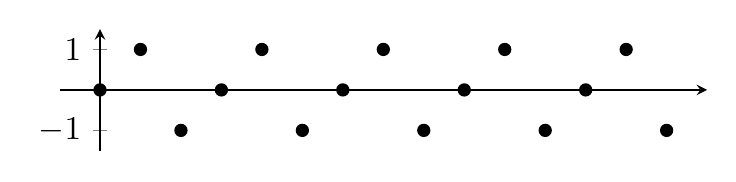
\begin{tikzpicture}[scale=1.2]
    \begin{axis}[
        xmin=-1,
        xmax=15,
        ymin=-1.5,
        ymax=1.5,
        xmajorticks=false,
        ytick={1, -1},
        yticklabels={$1$, $-1$},
        axis x line=center,
        axis y line=center,
        unit vector ratio*=1 1 1,
      ]
      \fill[black] (axis cs:0, 0) circle (2pt);
      \fill[black] (axis cs:1, 1) circle (2pt);
      \fill[black] (axis cs:2, -1) circle (2pt);
      \fill[black] (axis cs:3, 0) circle (2pt);
      \fill[black] (axis cs:4, 1) circle (2pt);
      \fill[black] (axis cs:5, -1) circle (2pt);
      \fill[black] (axis cs:6, 0) circle (2pt);
      \fill[black] (axis cs:7, 1) circle (2pt);
      \fill[black] (axis cs:8, -1) circle (2pt);
      \fill[black] (axis cs:9, 0) circle (2pt);
      \fill[black] (axis cs:10, 1) circle (2pt);
      \fill[black] (axis cs:11, -1) circle (2pt);
      \fill[black] (axis cs:12, 0) circle (2pt);
      \fill[black] (axis cs:13, 1) circle (2pt);
      \fill[black] (axis cs:14, -1) circle (2pt);
    \end{axis}
  \end{tikzpicture}
  \caption{The graph of Coppersmith's example.}
  \label{fig:coppersmith}
\end{figure}

Note that the closest linear function $g : \ZZ_m \to \ZZ_m$ to $f$ is given by $g(x) = 0$ for all $x \in \ZZ_m$, so $f$ is $2/3$-far from being linear. Note that $f$ fails for $x, y \in \ZZ_m$ with $x \equiv y \equiv 1 \pmod{3}$ or $x \equiv y \equiv 2 \pmod{3}$, and passes for all other $x, y \in \ZZ_m$. Therefore, the \emph{rejection probability of the linearity test} for $f$, denoted by $\delta_f$, is given by
$$ \delta_f = \PP_{x, y \in \ZZ_m}[f(x) + f(y) \neq f(x + y)] = \frac{2}{9}. $$
Fortunately, $2/9$ is the threshold; in other words, Coppersmith's example is the worst example. If $\delta_f < 2/9$ for some function $f : G \to G$ and finite group $G$, then $f$ must be $\delta_f$-close to being linear.

\section{Fourier Analysis for Boolean Functions}

The \emph{$n$-dimensional Boolean hypercube} $\{ 0, 1 \}^n$ can be interpreted as having $n + 1$ layers, where the $i^\text{th}$ layer consists of $n$-bit Boolean strings with $i$ ones for each $i \in \{ 0, \ldots, n \}$, and where two $n$-bit Boolean strings in consecutive layers are joined by an edge if they differ at exactly one bit. What are linear maps $\{ 0, 1 \}^n \to \{ 0, 1 \}$?

\begin{definition}
  Given $x, y \in \{ 0, 1 \}^n$, the \emph{inner product} of $x$ and $y$ is defined to be
  $$ x \cdot y = \sum_{i = 1}^n x_i y_i \pmod{2}. $$
\end{definition}

Note that addition modulo $2$ is the XOR operation. Linear functions on $\{ 0, 1 \}^n$ are of the form
\begin{align*}
  L_a(x) &= a \cdot x, && \text{for fixed $a \in \{ 0, 1 \}^n$}, \\
  \intertext{or, alternatively,}
  L_A(x) &= \sum_{i \in A} x_i \pmod{2}, && \text{for fixed $A \subset [n]$}.
\end{align*}
Therefore, there are exactly $2^n$ linear functions on $\{ 0, 1 \}^n$.

To simplify the presentation, we change the notation by letting $a \mapsto (-1)^a$ for $a \in \{ 0, 1 \}$ and by changing addition $a + b$ to multiplication $(-1)^a (-1)^b = (-1)^{a + b}$. Hence, the condition of linearity $f(a) + f(b) = f(a \oplus b)$ for all $a, b \in \{ 0, 1 \}^n$ is changed to $f(a) \cdot f(b) = f(a \odot b)$ for all $a, b \in \{ 1, -1 \}^n$, where $(x_1, \ldots, x_n) \oplus (y_1, \ldots, y_n) = (x_1 + y_1, \ldots, x_n + y_n)$ denotes the bitwise XOR (i.e., addition modulo $2$) of two $n$-bit Boolean strings, and $(x_1, \ldots, x_n) \odot (y_1, \ldots, y_n) = (x_1 \cdot y_1, \ldots, x_n \cdot y_n)$ denotes the bitwise multiplication of two $n$-bit $\{ 1, -1 \}$-valued strings. Moreover, linear functions on $\{ 1, -1 \}^n$ are of the form
\begin{align*}
  \chi_S(x) = \prod_{i \in S} x_i, && \text{for fixed $S \subset [n]$}.
\end{align*}

Now, the linearity test accepts if and only if $f(x) \cdot f(y) = f(x \odot y)$. Then
$$ f(x) f(y) f(x \odot y) = \left\{
  \begin{array}{ll}
    1, & \text{if the test accepts}, \\
    -1, & \text{if the test rejects}.
  \end{array}
\right. $$
Therefore, the indicator variable for the event that the test rejects is given by
$$ \mathds 1_{f(x) \cdot f(y) \neq f(x \odot y)} = \frac{1 - f(x) f(y) f(x \odot y)}{2} = \left\{
  \begin{array}{ll}
    0, & \text{if the test accepts}, \\
    1, & \text{if the test rejects}.
  \end{array}
\right. $$
This allows us to express the rejection probability in terms of the indicator variable:
$$ \delta_f = \PP_{x, y \in \{ 1, -1 \}^n}[f(x) \cdot f(y) \neq f(x \odot y)] = \EE_{x, y \in \{ 1, -1 \}^n}\left[\frac{1 - f(x) f(y) f(x \odot y)}{2}\right]. $$

\end{document}
